%----------------------------------------------------------
\def\notedate{2022.10.10}
\def\currentauthor{Василян А.Р. (РК6-73Б)}
%----------------------------------------------------------
\notestatement{rndhpcgui}{Метод построения оконного интерфейса пользователя на основе моделирования пользовательских целей}

%---------------------------------------------------------
\subsubsection{Ограничительный метод}
	
Для средств взаимодействия пользователя и ЭВМ с оконным интерфейсом типичным является ограничительный метод. Метод заключается в том, что пользователю предоставляется некий набор операций, благодаря которым он может выполнять определенные действия с описанными в ЭВМ объектами своей деятельности. Операция имеет название, исходные данные и результаты, представляющие собой объекты воздействия операции. Пользователь решает, какую из операций необходимо выбрать в данный момент для выполнения своего задания, выбирает нужную операцию и задает для нее исходные данные. После чего ЭВМ выполняет указанную операцию, активируя соответствующие функции приложения, и выдаёт результаты операции пользователю. 
	
	
По итогам выполнения очередной операции пользователь решает, какую следующую операцию ему нужно выбрать, передаёт ее ЭВМ на выполнение и т.д. Этот процесс он должен продолжать до тех пор, пока в итоге выполнения операций не будет достигнут желаемый результат, соответствующий выполненному заданию. Следовательно, пользователь должен сам планировать ход выполнения своего задания из предоставляемых ему операций. Обобщенная схема ограничительного метода взаимодействия приведена на рис.~\ref{rndhpcgui.2022.10.10.scheme1}. Для ограничительного метода считается, что у пользователя присутствуют процедурные знания, необходимые для планирования процесса выполнения своих заданий.

\begin{figure}[!ht]
  \centering
  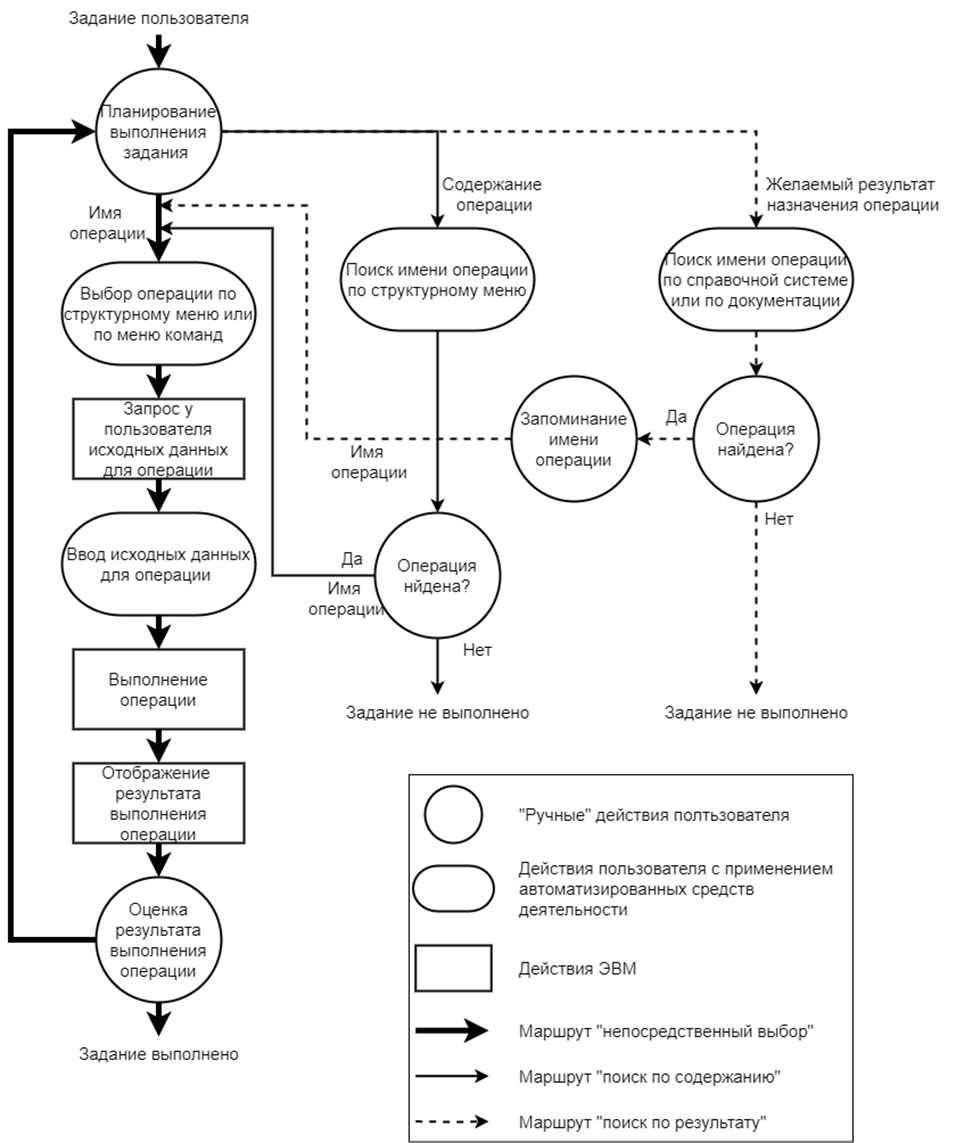
\includegraphics[scale=0.8]{ResearchNotes/rndhpc_int_gui_2022_10_10/scheme1.png}
  \caption{Обобщённая схема ограничительного метода взаимодействия <<пользователь-ЭВМ>> для оконного интерфейса}
  \label{rndhpcgui.2022.10.10.scheme1}
\end{figure}

\subsubsection{Направляющий метод}
	
DT-модель (ДТ -- диалоговая транзакция) диалога является основой направляющего метода взаимодействия пользователя с ЭВМ для оконного интерфейса. 
	
Цели партнеров в диалоге делятся на практические цели (ПЦ) и коммуникативные цели (КЦ). ПЦ -- это описание определенной ситуации в общей предметной области партнеров, которую (ситуацию) один из партнеров (инициатор ПЦ) стремится достичь с помощью другого партнера. КЦ -- это намерение партнера-инициатора ПЦ довести свою ПЦ до сведения второго партнера. При построении DT-модели в качестве целей партнеров в диалоге рассматриваются только ПЦ. пользователя является представлением его задания в ЭВМ. ДТ описывает часть процесса диалога, ограниченную выдвижением и обработкой некоторой ПЦ. Выделяются элементарные ДТ (ЭДТ) и неэлементарные ДТ. ЭДТ является минимальным структурным элементом описания процесса диалога в DT-модели. ЭДТ представляет собой последовательность действий (речевых актов), совершаемых поочередно партнерами по диалогу и направленных на выдвижение и обработку элементарной ПЦ. ЭДТ состоит из трех фаз:
\begin{enumerate}
	\item Выдвижение элементарной ПЦ партнером-инициатором и передача ее партнеру-исполнителю.
	\item Реагирование на ПЦ, т. е. формирование партнером-исполнителем положительной или отрицательной реакции на выдвинутую цель и передача реакции инициатору ПЦ.
	\item Оценивание реакции партнером-инициатором (принять ее или отклонить с точки зрения соответствия реакции выдвинутой ПЦ) и передача оценки исполнителю.
\end{enumerate}

	
Пример ЭДТ представлен на рис.~\ref{rndhpcgui.2022.10.10.example}.
\begin{figure}[!ht]
  \centering
  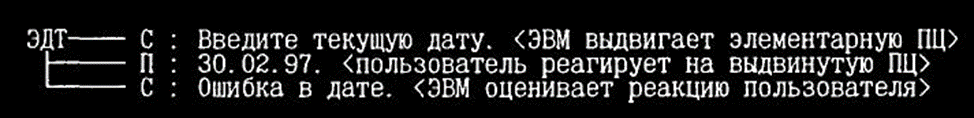
\includegraphics[scale=0.8]{ResearchNotes/rndhpc_int_gui_2022_10_10/example.png}
  \caption{Пример ЭДТ}
  \label{rndhpcgui.2022.10.10.example}
\end{figure}

	
В отличие от ограничительного метода взаимодействия, направляющий метод основан на описании в ЭВМ модели пользовательского задания как цели. Каждая из целей соответствует определенному пользовательскому заданию, которое может выполнить ЭВМ во взаимодействии с пользователем. Выбор и целенаправленное упорядочивание подзаданиями, приводящих к выполнению пользовательского задания, совершает не пользователь, а ЭВМ. От пользователя требуется в ответ на запросы ЭВМ ввести исходные данные, необходимые для этих операций.

	
Направляющий метод взаимодействия <<пользователь-ЭВМ>> состоит из следующих основных этапов:
\begin{itemize}
	\item информирование пользователя о множестве допустимых заданий, которые может выполнять ЭВМ в рамках данного приложения;
	\item выбор пользователем задания по меню заданий и передача его ЭВМ на выполнение;
	\item планирование процесса взаимодействия при выполнении задания;
	\item ввод пользователем данных, необходимых ЭВМ для выполнения задания;
	\item передача пользователю результатов выполнения задания и их оценка пользователем. 
\end{itemize}

Обобщенная схема направляющего метода взаимодействия приведена на рис.~\ref{rndhpcgui.2022.10.10.scheme2}. В соответствии с этой схемой пользователь должен выбрать в меню заданий свое задание и передать его ЭВМ на выполнение. Выбранное задание рассматривается в ЭВМ как цель пользователя. Достижение этой цели обеспечивается в ходе последующего диалога с пользователем, в котором инициатива взаимодействия принадлежит ЭВМ.

\begin{figure}[!ht]
  \centering
  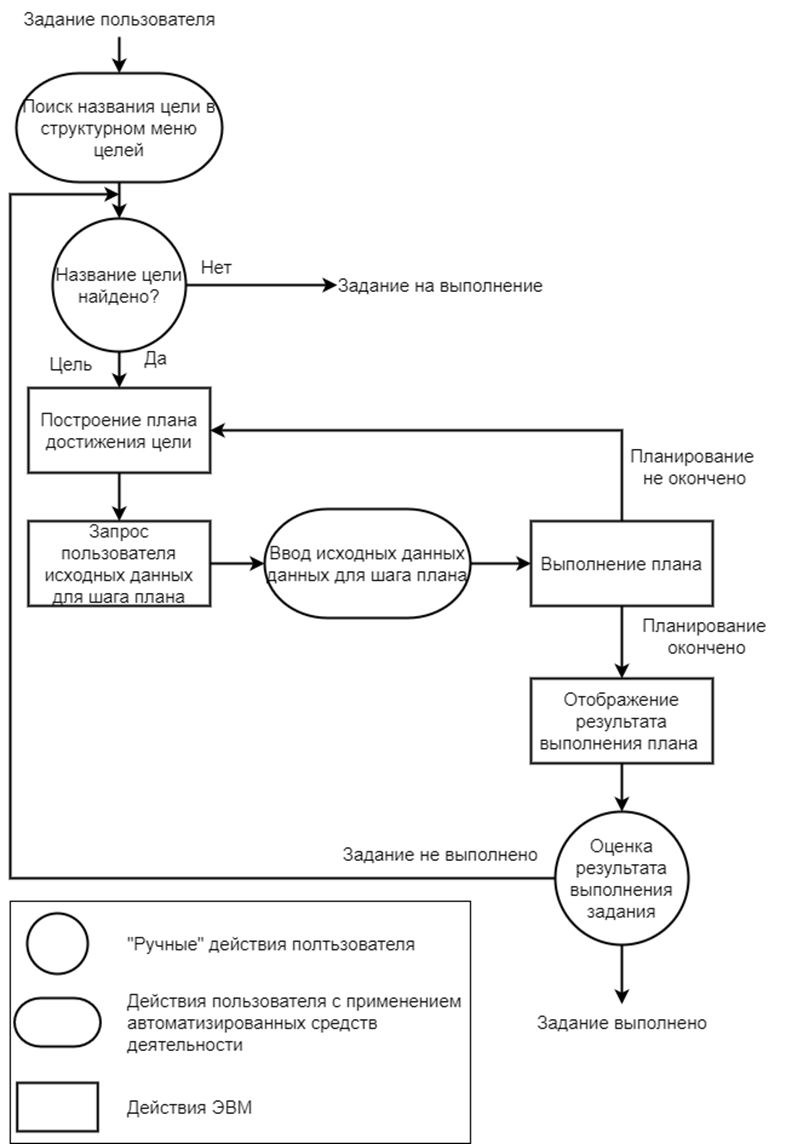
\includegraphics[scale=0.8]{ResearchNotes/rndhpc_int_gui_2022_10_10/scheme2.png}
  \caption{Обобщённая схема направляющего метода взаимодействия "пользователь-ЭВМ" для оконного интерфейса}
  \label{rndhpcgui.2022.10.10.scheme2}
\end{figure}

	
В отличие от схемы ограничительного метода, в рассматриваемой схеме существует только один маршрут движения, т. е. здесь нет зависимости результата от степени пользовательской подготовки. После передачи пользовательской цели в ЭВМ дальнейшее взаимодействие не требует инициативы пользователя вплоть до этапа оценки результата достижения цели. Планирование процесса взаимодействия на множестве ДТ осуществляет ЭВМ в соответствии с DT-моделью диалога. Данные, необходимые ЭВМ для достижения принятой от пользователя цели, вводятся пользователем только по запросу, т.е. на этой стадии он выступает в роли реагирующего партнера.

	
Итак, главное отличие направляющего метода взаимодействия <<пользователь-ЭВМ>> по сравнению с ограничительным методом состоит в том, что инициатива взаимодействия по достижению цели пользователя принадлежит не пользователю, а ЭВМ. Это означает, что ЭВМ играет активную роль в целенаправленном взаимодействии по выполнению задания пользователя. Сопоставление схемы направляющего метода взаимодействия (рис.~\ref{rndhpcgui.2022.10.10.scheme2}) со схемой ограничительного метода (рис.~\ref{rndhpcgui.2022.10.10.scheme1}) позволяет наглядно судить об упрощении работы пользователя за счет того, что пользователю уже не требуется знать, как выполнить то или иное задание, поскольку планирование процесса взаимодействия выполняет не он сам, а ЭВМ.
%----------------------------------------------------------
% Атрибуты задачи
\noteattributes{}
%----------------------------------------------------------

